\section{同変Schubert計算}
\subsection{Grassmann多様体の同変コホモロジー}
$\text{Gr}_k(\complex^n)=\set{V\subset \complex^n}{\dim V = k}$をGrassmann多様体という.$T=\complex^n$とするとき,$T$は$\complex^n$に
\[
(t_1,\cdots,t_n)\cdot(x_1,\cdots,x_n)=(t_1x_1,\cdots,t_nx_n)
\]
によって左から作用する.この作用は自然に$\text{Gr}_k(\complex^n)$への作用を誘導し,$\text{Gr}_k(\complex^n)$は$T$空間となる.$\text{Gr}_k(\complex^n)$の$T$同変コホモロジーの構造は組み合わせ的に決定することができる.
$\binom{n}{k}$を$0$と$1$からなる$n$文字の文字列のうち,$1$が$k$個使われている文字列の集合とする.$\lambda=\lambda_1\cdots \lambda_n\in\binom{n}{k}$に対して置換$\sigma\in\mathfrak{S}_n$の$\binom{n}{k}$への作用を$\sigma\lambda=\lambda_{\inv{\sigma}(1)}\cdots\lambda_{\inv{\sigma}(n)}$で定める.
$\lambda=\lambda_1\cdots \lambda_n\in\binom{n}{k}$に対して,
\[
\Omega_\lambda^\circ=\set{V\in \text{Gr}_k(\complex^n)}{\dim(V\cap F_i)= \dim(\complex^\lambda\cap F_i),\quad \forall i\in \set{1,\cdots n}{}}
\]
をSchubert cellという. ここで,$\complex^\lambda=<\lambda_1e_1,\cdots,\lambda_ne_n>$, $F_i=<e_{n-i+1},\cdots,e_n>$である. 

\begin{prop}
  $\text{inv}(\lambda)=\set{(i,j)}{\lambda_i=1, \lambda_j=0, i<j}$とすると$\Omega_\lambda^\circ$は$\complex^{|\text{inv}(\lambda)|}$に同相であり
\[
\text{Gr}_k(\complex^n)=\bigsqcup_{\lambda\in\binom{n}{k}}\Omega_\lambda^\circ
\]
となる.
\end{prop}

\begin{proof}
  
\end{proof}

したがって$H^*(\text{Gr}_k(\complex))$は$\Omega_\lambda^\circ$の定めるホモロジー類のPoincare双対$S_\lambda$たちで$\integer$上生成される. $\text{Gr}_k(\complex)$はequivariantly formalであるから$H^*_T(\text{Gr}_k(\complex^n))$は$H^*_T(\text{pt})=\integer[y_1,\cdots,y_n]$上$S_\lambda$たちで生成される. $S_\lambda$をSchubert classという.

$2$つのSchubert classの積$S_\lambda S_\mu$を$\{S_\nu\}_{\nu\in\binom{n}{k}}$の$\integer[y_1,\cdots,y_n]$係数の線形結合で
\[
S_\lambda S_\mu=\sum_{\nu\in\binom{n}{k}}C^\nu_{\lambda\mu}S_\nu
\]
このように表したとき,この係数$C^{\nu}_{\lambda\mu}$を計算する組み合わせ的手法を紹介することが本論文の目的である.


\subsection{GKM条件によるSchubert Classの特徴づけ}

$\text{Gr}_k(\complex^n)$の$T$作用における固定点は$\{\complex^\lambda\}_{\lambda\in\binom{n}{k}}$であるから,[GKM]より$H^*_T(\text{Gr}_k(\complex^n))$は$\bigoplus_{\lambda\in\binom{n}{k}}H^*_T(\text{pt})$の部分代数である.GKMの定理を適用するために$\text{Gr}_k(\complex^n)$の$T$不変な$\mathbb{CP}^1$を計算する.

\begin{prop}
  $\lambda,\mu\in\binom{n}{k}$に対して$\complex^\lambda$と$\complex^\mu$を結ぶ$T$不変な$\mathbb{CP}^1$が存在するための必要十分条件は, ある$(i, j)\in\text{inv}(\lambda)$に対して$\mu = (i, j)\lambda$
  となっていることである.
\end{prop}

\begin{proof}
  
\end{proof}






\subsection{Schubert puzzleによる方法}

\begin{theo}
  以下の$8$種類の図形をpuzzle pieceと呼ぶ.
  \begin{align*}
    \begin{tikzpicture}
      \coordinate (A) at (0,0);
      \coordinate (B) at (2,0);
      \coordinate (C) at (1,1.7);
      \draw (A)--(B)--(C)--cycle;
      \coordinate(P) at (3,0);
      \draw ($(A)+(P)$)--($(B)+(P)$)--($(C)+(P)$)--cycle;
      \coordinate(Q) at (6,0);
      \draw ($(A)+(Q)$)--($(B)+(Q)$)--($(C)+(Q)$)--cycle;
    \end{tikzpicture}\\
    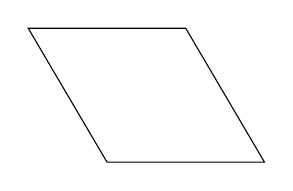
\begin{tikzpicture}
      \draw (0,0)--(2,0)--(1,1.7)--(-1,1.7)--cycle;
    \end{tikzpicture}
\end{align*}
\end{theo}



\subsection{edge labeled tableauxによる方法}

\begin{defin}
  $n$の分割$\lambda=(\lambda_1\geq\cdots\geq\lambda_k>0)$に対して,$1$行目に$\lambda_1$個の箱を, $2$行目に$\lambda_2$個の箱を,順に$k$行目まで左寄せで書いた図をYoung図形という.以降分割とYoung図形を同一視して同じ記号で表す. $\lambda$の各箱に,各行について左から右に単調増大, 各列について上から下に単調増大となるように相異なる数字を書き入れたものをstandard tableauxという. 

\[
\ytableausetup{nobaseline}
\ydiagram{4, 3, 3, 1}
\quad\begin{ytableau}
    1&4&5&6\\
    2&3&8\\
    7&9&10\\
    \text{ab}
\end{ytableau}
\]

\end{defin}

\begin{defin}
  分割$\lambda, \mu$に対して,$\lambda<\mu\Leftrightarrow \lambda_i<\mu_i\:(\forall i)$によって順序を定める. $\lambda<\mu$を満たすYoung図形に対して,$\mu$のYoung図形から$\lambda$に相当する部分を取り除いた図形を歪Young図形といい.$\mu/\lambda$で表す. 整数$n>0$を固定する. 歪Young図形の各箱に$1$から$n$までの数字を書き入れ,水平方向の各辺に$\{1,\cdots,n\}$の部分集合(空でもよい)を書き入れたものを, equivariant fillingという. equivariant fillingのうち,ラベルに関して次の条件を満たすものをequivariant standard tableauxという.
  \begin{itemize}
    \item $1$から$n$までの各数字が,いずれかの箱のラベルに現れるか,またはいずれかの辺のラベルの要素になっている.また$1$から$n$までの各数字がちょうど1回しか現れない.
    \item 各箱のラベルについて,左隣の箱のラベルよりも大きい
    \item 各箱のラベルについて,上辺のラベルが空でないなら,その最大値よりも大きい. 空であるならば,すぐ上の箱のラベルより大きい
    \item 各辺のラベルについて,そのすべての数字がすぐ上の箱に書かれたラベルよりも大きい
  \end{itemize}
  形が$\mu/\lambda$で$1$から$n$までの数字が書かれたequivariant standard tableauxの全体を$\text{EqSYT}(\mu/\lambda, n)$とする.
\end{defin}

\begin{defin}
  $\lambda$の箱xが$T\in\text{EqSYT}(\mu/\lambda, n)$の内隅であるとは,$x$のすぐ右とすぐ下の箱が$\lambda$の箱でないことをいう.また$\mu/\lambda$の箱$x$が外隅であるとは,$x$のすぐ右とすぐ下の箱が存在しないことをいう.$T$の内隅$x$に対して,次の操作を考える:
  \begin{enumerate}
    \item $x$の下辺のラベル$l$が空でないなら,$l$の最小値を$x$のラベルに移す
    \item $x$の下辺のラベルが空であるとし,$x$のすぐ右の箱を$y$,すぐ下の箱を$z$とする.$y$と$z$のうち,ラベルの小さい方の箱を$x$と交換する(このとき辺のラベルは交換しない).
  \end{enumerate}
  (i)の操作が行われる,もしくは$x$が外隅になるまで(i),(ii)を繰り返してできるtableauxを$\text{EqJdt}_x(T)$とする.
\end{defin}

\begin{defin}
  $\lambda$の箱を下から上,右から左に順番に数えて$x_1,\cdots,x_m$とする.$T\in\text{EqSYT}(\mu/\lambda, n)$に対して,$T$のequivariant rectificationを
  \[
  \text{EqRect}(T)=\text{EqJdt}_{x_m}(\text{EqJdt}_{x_{m-1}}(\cdots(\text{EqJdt}_{x_1}(T))\cdots))
  \]
  とする.
\end{defin}

次に$T\in\text{EdSYT}(\mu/\lambda, n)$に対してそのウェイトを定義する.

\begin{defin}
  正の整数$m, k$を$m>k$とする.$\Lambda=(m,\cdots,m)$とする.$\Lambda$の箱$x$に対して
  \[
  \beta(x)=t_{i+1}-t_i
  \]
  とする.ここで$i$は$\Lambda$の右上の隅の箱から$x$までのManhattan距離である.
  \[
  \begin{ytableau}
    4 & 3 & 2 & 1\\
    5 & 4 & 3 & 2\\
    6 & 5 & 4 & 3
  \end{ytableau}
  \]
\end{defin}

\begin{defin}
  $T\in\text{EqSYT}(\mu/\lambda, n)$を固定し,$l$を$T$の辺のラベルに含まれる要素とする.$\text{factor}(l)$を次のように定義する.
  \begin{enumerate}
    \item $l$が含まれる列をrectificationしたあとも$l$が辺のラベルであるなら$\text{factor}(l)=0$とする.
    \item $l$が含まれる列のrectificationにおいて,$l$が通った箱を下から順に$x_1,\cdots,x_s$とする.$x_s$と同じ行で$x_s$の右側にある$T$の箱を左から順に$y_1,\cdots,y_t$とする.このとき$\text{factor}(l)=\beta(x_1)+\cdots+\beta(x_s)+\beta(y_1)+\cdots+\beta(y_t)$とする.
  \end{enumerate}
\end{defin}

\begin{defin}
  $T\in\text{EqSYT}(\mu/\lambda, n)$に対して
  \[
  \text{wt}(T)=\prod_{l:\text{edge label}}\text{factor}(l)
  \]
  とする.
\end{defin}

\begin{theo}
  \[
  C^{\nu}_{\lambda,\mu}=\sum_{T\in\text{EqSYT}(\nu/\lambda, |\mu|)}\text{wt}(T)
  \]
  が成り立つ.
\end{theo}




\subsection{weight preserving bijectionの構成}